%%=============================================================================
%% Methodologie
%%=============================================================================

\chapter{\IfLanguageName{dutch}{Methodologie}{Methodology}}
\label{ch:methodologie}

%% TODO: Hoe ben je te werk gegaan? Verdeel je onderzoek in grote fasen, en
%% licht in elke fase toe welke stappen je gevolgd hebt. Verantwoord waarom je
%% op deze manier te werk gegaan bent. Je moet kunnen aantonen dat je de best
%% mogelijke manier toegepast hebt om een antwoord te vinden op de
%% onderzoeksvraag.

Aan de hand van verchillende RPA providers zal een concreet proces geautomatiseerd worden op Metamaze, het automated document processing platform bij Faktion zelf. De code voor de verschillende workflows en packages geschreven voor dit onderzoek zijn te vinden op GitHub\footnote{https://github.com/MoutPessemier/BachelorProef}.


\section{Voorbereiding}
%Ter voorbereiding van het te automatiseren proces bij Faktion heb ik mij eerst ingewerkt op het platform waar dit proces zich voordoet. Ook heb ik de volledige 'RPA Developer Essentials' cursus aangeboden door UiPath gevolgd om een algemene basiskennis rond RPA te beheersen. Daarna is de afweging gemaakt welke RPA software providers nu zullen vergelijken worden. Hieruit zijn 5 kandidaten naar boven gekomen. Als 2 grote providers zal gekeken worden naar UiPath en Automation Anywhere. Voor de kleinere providers wordt gekeken naar AutomationEdge en WorkFusion.

%Ondertussen werd het te automatiseren proces uitgewerkt. Dit proces zal worden geïmplementeerd op de verschillende  platformen. Het gaat hier over het schrijven van een eigen activiteit die in verschillende workflows kan gebruikt worden om te werken met het Metamaze platform.

Eerst en vooral is het MetaMaze platform, gebouwd door Faktion, gronding geëxploreerd geweest. Zo werd een nieuw project aangemaakt, werden er documenten geüpload en gelabeld om een model te kunnen trainen. Nadien werd dit model dan gebruikt om voorspellingen te doen op nieuwe, soortgelijke documenten. Hierbij werd soms expres een verkeerd document geüpload om ook de 'manual intervention' te testen en kijken hoe dit eventueel in een proces kan gegoten worden. Op basis hiervan is een algemeen voorbeeld proces ineen gestoken geweest.

\begin{figure}[h]
	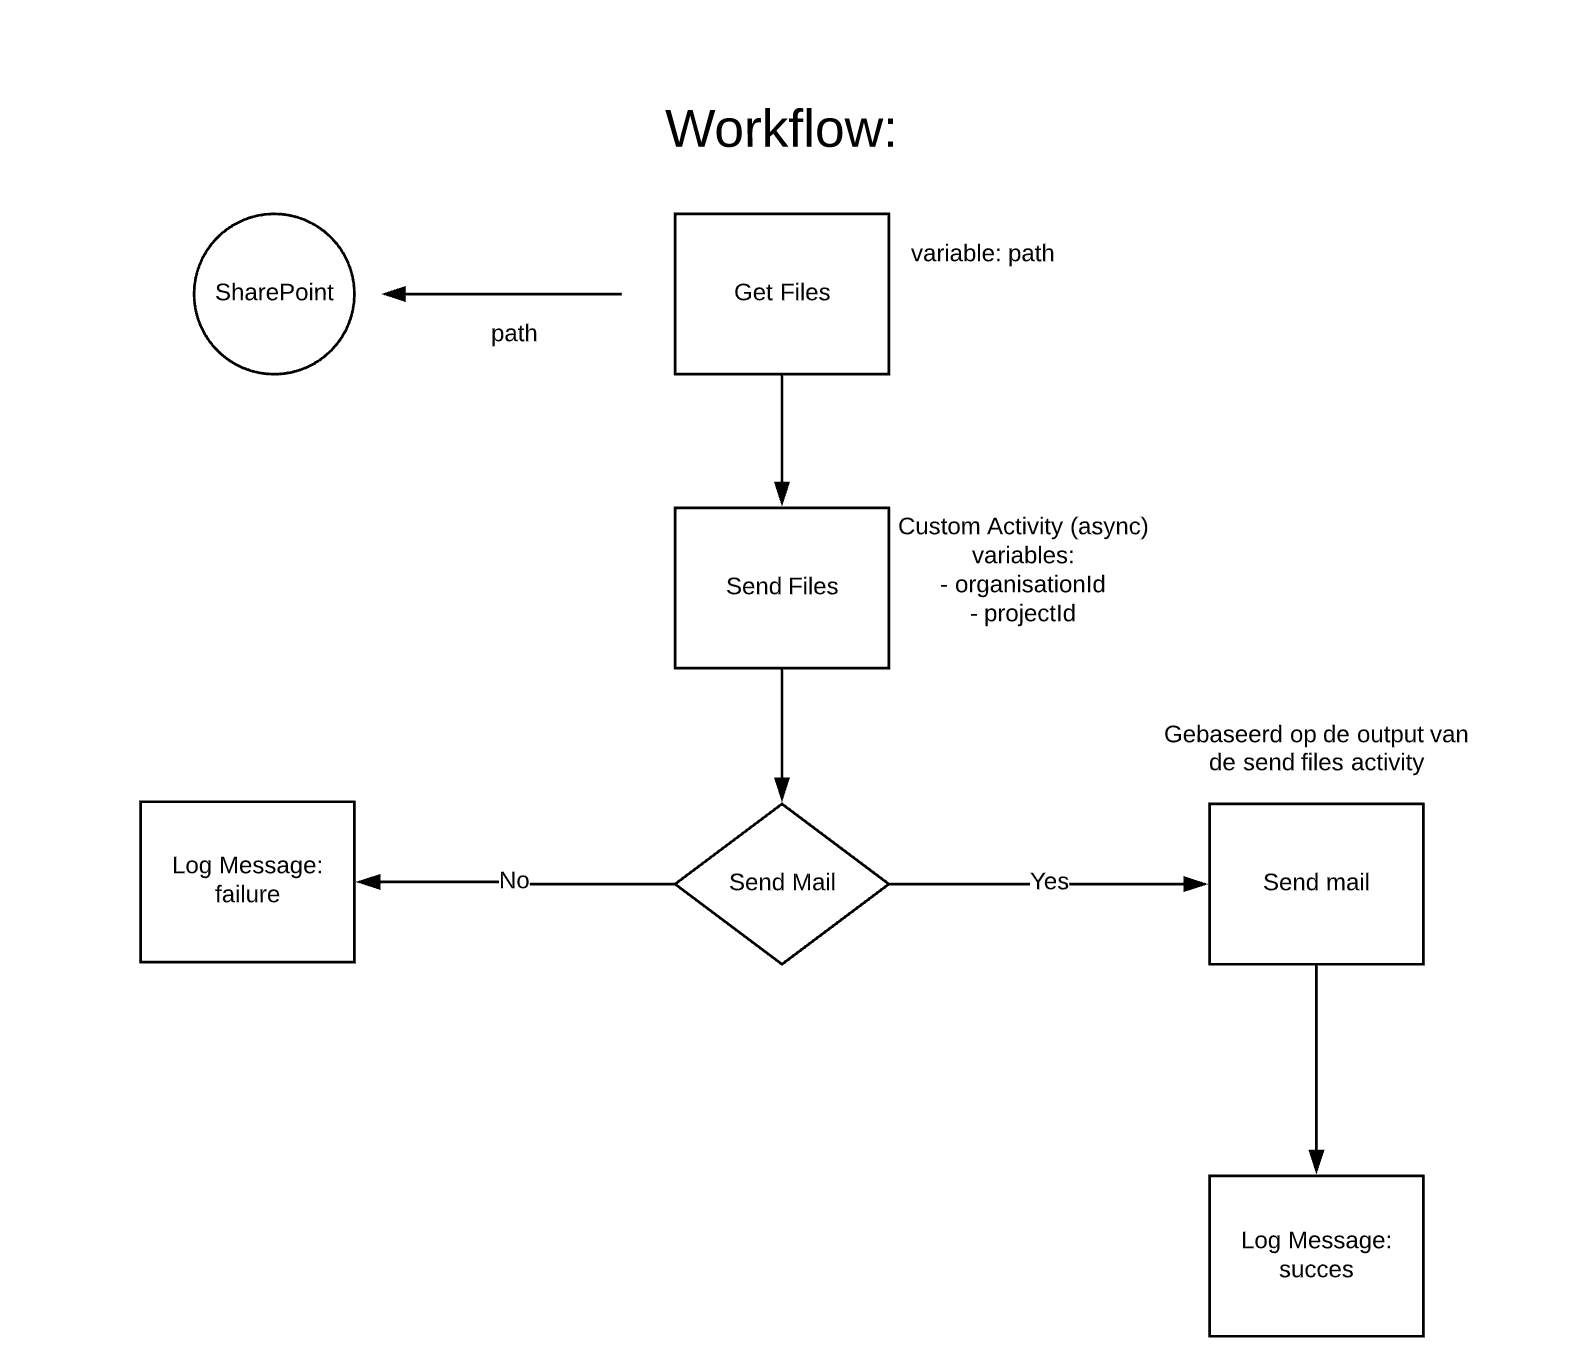
\includegraphics{exampleProcess.png}
	\caption{Voorbeeldproces dat gebruik maakt van de custom Send Files activiteit.}
\end{figure}

Het algemeen proces dat zal geautomatiseerd worden op de verschillende RPA solutions gaat als volgt te werk: Eerst wordt vanuit een bepaald punt (folder op de computer, OneDrive, DropBox, SharePoint) een aantal files opgehaald. Deze files worden doorgegeven aan een zelfgeschreven activiteit. In deze activiteit zullen deze files verstuurd worden naar de MetaMaze API. Nadien wordt er gewacht tot een antwoord terug komt van de server met de resultaten van de upload. Deze resultaten worden terug gegeven naar de volgende stap in de workflow. Door verder te weken met de resulterende JSON kan gekeken worden of de zekerheid waarmee een bepaalde entity dat uit een document is gehaald, onder de minimum zekerheid (threshold) zit of niet. Als er geen onder de threshold zitten wordt het proces afgesloten met een gepaste melding. Als er 1 of meerdere confidence scores onder de threshold zitten zal eerst een mail verstuurd worden naar de klant om te laten weten welke entities de minimum niet gehaald hebben voor dat het proces eindigt met een gepaste melding.

\subsection{Criteria}
De criteria die onderzocht zijn kunnen opgedeeld worden in 3 categorieën: technische criteria, bedrijfscriteria en financiële criteria. Onder de technische criteria valt de mogelijkheid om gemakkelijk zelfgeschreven activiteiten toe te voegen, [...]. Onder bedrijfscriteria vinden we het feit of er een grote onderneming achter het platform staat, hoe actief de community is van het platform, hoe de klantservice is. Tot slot valt onder de financiële categorie natuurlijk de prijs van een enterprise versie maar daarnaast ook of er een mogelijkheid is om een community editie te gebruiken en hoe uitgebreid deze versie is.

De nadruk wordt hier gelegd op een integratie met een eigen API, op een eigen webplatform.

De verschillende criteria hebben elk een zwaarte toegekend gekregen. Hierop worden ze gescoord en op het einde worden alle punten opgeteld.

\subsubsection{Puntenverdeling}
Technische Criteria
\begin{itemize}
	\item Custom activities/implementations --> is de mogelijkheid er om een eigen code toe te voegen. Als die er is, hoe uitgebreid is dit, enkel als script of ook volwaardige activiteiten: /5
	\item Herbruikbaarheid --> kunnen bepaalde (zelfgemaakte) workflows/activities hergebruikt worden door jezelf en/of anderen: /3
	\item Tools --> Hoe zit het met de tools om een workflow op te zetten: /5
	\item Bot management --> hoe zit het met het managen van de bots. Hoe gebeurd dit en kan dit op een eenvoudige manier: /3
	\item IPA capaciteiten --> kan AI en ML makkelijk geïntegreerd worden in de workflow om IPA te bereiken. Wat wordt aangeboden door de provider zelf: /3
\end{itemize}

Bedrijfscriteria
\begin{itemize}
	\item Community --> hoe actief zijn ze op het forum, hoe groot is de community: /5
	\item Weblessen --> worden weblessen aangeboden door de provider en wat is de kwaliteit van deze lessen: /3
	\item Support --> hoe is het contact met de organisatie: /3
\end{itemize}

Financiële criteria
\begin{itemize}
	\item Prijs --> Wat is de prijs is het platform: /3
	\item Community edition --> hoe uitgebreid en representatief is deze versie ten opzichte van de enterprise edition: /5
\end{itemize}

Dit komt uit op een totale score van 37.

\section{Implementatie}

\section{Beoordeling}
\subsection{UiPath}
Bij UiPath is het mogelijk om in de community edition custom activities toe te voegen. Hiervoor moet een C\# Class Library gemaakt worden. Van dit project moet nadien een NuGet Package gemaakt worden en lokaal toegevoegd worden aan UiPath om toegang te krijgen tot deze activiteit. Het nadeel hierbij is dat elke wijziging in code een nieuwe versie van de package voorstelt die opnieuw moet worden gepubliceerd. (4.5/5)

Voor de herbruikbaarheid van custom activities en workflows kan gebruikt worden van de orchestrator in combinatie met de market place. Packages kunnen gepubliceerd worden naar de orchestrator en deze kunnen op die manier ter beschikking gesteld worden op de market zodat anderen deze package kunnen hergebruiken. Het is ook mogelijk om workflow bestanden te gaan aanroepen binnen andere workflows. (3/3) 

De beschikbare tool voor het implementeren van een workflow is UiPath Stuido, een ide die zich focust op het ontwerpen en uitwerken van een workflow. Hierbinnen kan niet geprogrammeerd worden, daarvoor moet beroep gedaan worden op een C\# ide zoals Visual Studio. De tool zelf voelt heel intuïtief aan en zit logisch ineen. Het is makkelijk om een workflow op te bouwen en er zijn ook features aanwezig om de workflow te debuggen. (5/5)

Het managen van de UiPath bots gebeurd aan de hand van het online platform, de UiPath Orchestrator. Hierop worden machines vastgelegd waarop een bot attended of unattended kan gaan werken, worden bots gedeployed, taken ingepland, queues opgezet en assets bewaard en analytics weergegeven. Kortom, alles wat nodig is om de verzameling bots te gaan managen op een professionele manier. Het platform zit logisch ineen en werkt uitstekend. (3/3)

[IPA]

De community achter UiPath is groot en actief. Het forum wordt gebruik door zowel UiPath zelf om belangrijke mededelingen te maken, als door de klanten die er terecht kunnen met vragen over allerhande topics. (5/5)

De lessen die aangeboden worden door UiPath zitten zeer goed ineen. Alles wordt rustig opgebouwd, de video's zijn duidelijk en makkelijk te volgen en er zijn voldoende oefeningen om de net geleerde skills eens te testen. (3/3).

Support zit ook goed. Ze zijn makkelijk te bereiken via ofwel het forum ofwel via mail waarop er binnen de 1-2 dagen wordt geantwoord. (3/3)

[PRIJS]

De community edition van UiPath als platform is zeer uitgebreid. In Studio kan je alles wat ook mogelijk is in de enterprise versie. Het grote verschil ligt hem in de Orchestrator. Hirbij wordt dit een on-premise (geïnstalleerd op de machine van de host) of cloud-hosted Orchestrator waarbij er een oneindig aantal robots kan gemaakt worden. Ook kunnen er meerdere soorten bots gemaakt worden. Ook wordt toegang verleend tot premium support en is er de mogelijkheid om up/down te scalen met wat nodig is binnen het bedrijf. (3/3)

Dit brengt de totale score van UiPath op 29.5/37.

\subsection{Automation Anywhere}
Automation Anywhere staat niet toe om een custom activity te gebruiken in de community edition. Alles moet geautomatiseerd worden met de standaard activiteiten. Dit aanbod is wel uitgebreider dan bij UiPath. [...] (3/5)

De herbruikbaarheid [...] (/3)

De tools die gebruikt worden om een workflow te implementeren zijn allemaal cloud-based. Op de site wordt de flow opgebouwd en nadien wordt verbinding gemaakt met het lokaal apparaat waarop de workflow getest kan worden. De tool is over het algemeen begrijpbaar maar voor eenzelfde stap in UiPath, zijn geregeld meerdere stappen nodig in Automation Anywhere. Er is ook een mogelijkheid om de workflow te debuggen. (4/5)

Voor de bots te managen moet bij Automation Anywhere niet ver gegaan worden. Dit zit namelijk in het zelfde webplatform als het maken van de robots. Hier kunnen robots gestart worden om taken uit te voeren op bepaalde machines. Er zijn geen verschillende typen van bots. [explore further!] (1.5/3)

Voor het maken van AI en ML bots kan beroep gedaan worden op de IQBot van Automation Anywhere. Hier wordt de focus gelegd op automated document processing (ADP) wat exact hetzelfde is als MetaMaze. Dit getrainde model kan dan gebruik worden in een gewone flow. Daarnaast zijn er ook nog enkele standaard activiteiten die werken met NLP en OCR. (2.5/3)

De community achter Automation Anywhere is groot en actief al worden er geen updates gepost door Automation Anywhere zelf. Ook hier wordt gebruik gemaakt van duidelijke subcategorieën om de posts in op te delen. (4.5/3) 

Er is een zeer ruim aanbod aan lessen voor verschillende onderdelen van het RPA development proces. Dit gaat van de voorbereiding tot het verstaan van de business needs en het implementeren van een proces. De video's zijn duidelijk opgebouwd in een cursus structuur en zijn makkelijk te volgen. (3/3)

Support zit zeer goed. Contact via mail of telefoon is rap gelegd en er wordt een inspanning geleverd om zo goed en snel mogelijk hulp te bieden op de verschillende vragen of problemen. (3/3)

[PRIJS]

De community edition van Automation Anywhere is uitgebreid genoeg tot het punt waar de beslissing om voor dit platform te kiezen kan gemaakt worden maar langs de andere kant steekt ook veel weg achter de premium versie. [...] (/5)

Dit levert Automation Anywhere een score op van 21.5/37.

\subsection{WorkFusion}

Er is geen mogelijkheid om een custom activity toe te voegen in beide versies. Wel kan een custom script geschreven worden dat code kan uitvoeren. Dit script is geschreven in Groovy en kan alleen gebruik maken van de basic Groovy onderdelen. Geen andere jars kunnen toegevoegd worden wat resulteert in zeer beperkte mogelijkheden om een eigen iets te gebruiken. (1.5/5)

Herbruikbaarheid bij WorkFusion kan gevonden worden in de recordings. Deze kunnen hergebruikt worden waarbij alleen de parameters moeten/kunnen aangepast worden. [...] (1.5/3)

De WorkFusion tools om een recording te maken bestaat uit een dedicated ide waar zowel in kan geprogrammeerd worden als een recording opgebouwd worden. Het grootste probleem bij het programmeer gedeelte is dat er geen syntax highlighting of autocomplete is. Er moet dus feitelijk blind geprogrammeerd worden. Daarom dat meestal andere ide's gebruikt worden zoals IntelliJ. Langs de recorder kant ziet de ide er zeer droog uit. De UI is niet aantrekkelijk en er zijn ook maar een beperkt aantal standaard activiteiten voorzien. (1/5)

Bot management gebeurd bij WorkFusion aan de hand van een online platform genaamd Watch Tower. [...] (/3)

De IPA capaciteiten binnen de recording zijn zeer beperkt. Er wordt niets aangeboden rond AI of ML, noch rond NLP. Wel kan gebruik gemaakt worden van OCR. Andere AI en ML solutions zitten vast achter een premium account. (1/3)

De community is klein en inactief. Er gebeurd niet veel op het forum en de weinige vragen die gesteld worden, worden meestal niet opgelost. (1/5)

Er worden online lessen aangeboden maar deze zijn beperkt en niet altijd even diepgaand. Het is een start maar er mag zeker nog meer/uitgebreid worden. (1/3)

[Support]

[PRIJS]

De community edition van WorkFusion bevat enkel de ide, geen toegang tot de Watch Tower. Daarnaast geeft een premium versie ook een credential manager, task scheduler, meerdere parallel lopende bots, ML capaciteit en geavanceerde analytics. (2.5/5)

Alles opgeteld komt dit uit op 9.5/37 voor WorkFusion.

\subsection{Intellibot}

Custom activities zijn zeer gemakelijk te schrijven voor IntelliBot en dit alles dan ook nog eens binnen de community editie. Er moet niet gebuild en gepubliceerd worden tot een package, de .dll file kan rechtstreeks gebruikt worden. Daarnaast is er ook nog eens de mogelijkheid om een script toe te voegen als een volledige class library niet nodig is. (5/5)

[Herbruikbaarheid]

De tools gebruikt om een workflow te bouwen in IntelliBot is hun eigen ide, IntelliBot Studio. Hierin kan niet geprogrammeerd worden. Het opbouwen van de workflow is totaal anders als de rest. Bij de andere providers was het altijd in sequentie op te bouwen en was het duidelijk welke activiteit volgt uit welke. Bij IntelliBot is dit een pak minder overzichtelijk. Hier wordt gebruik gemaakt van lijnen om activiteiten met elkaar te verbinden en zo de workflow op te bouwen. Van zodra een activiteit met veel input en output gebruikt wordt, dan wordt het rap een warboel van lijnen die door elkaar getrokken worden. Hierdoor is het makkelijk om het overzicht te verliezen. (2.5/5)

Ook IntelliBot heeft zoals UiPath een web platform, de Orchestrator, waarop het managen van de bots plaats vindt. Beide platformen lijken op elkaar, al is die van UiPath uitgebreider en ook iets beter ineen gestoken. (2/3)

[IPA]

De IntelliBot community is net zoals WorkFusion beperkt maar in tegenstelling tot WorkFusion is deze wel actief. De werknemers van IntelliBot volgen het forum op en antwoorden ook op de verschillende vragen. (3.5/5)

De lessen aangeboden op het platform zijn inhoudelijk diepgaand genoeg maar zeer beperkt in aantal. (2/3)

De support is zeer goed bij IntelliBot. Ze focussen zich op de individuele klant in plaats van de massa wat soms het geval is bij de grote providers. Feedback en hulp op maat en binnen 1-2 dagen is dan ook geen verrassing. (3/3)

[PRIJS]

De community editie bevat voor de IntelliBot Studio bijna elke feature. Het enigste wat vergrendeld zit achter de enterprise edition, is het maken van chatbots. Aan de andere kant is de orchestrator wel onderhevig aan grote wijzigingen. Zo kan je een bot alleen lokaal draaien in de comunity editie. Voor het inplannen van taken en het toekennen van jobs aan bots moet een premium license gekocht worden. Zelf raden ze aan om de community editie te gebruiken voor het maken en testen van robots en de enterprise editie te kopen van zodra ze naar productie moeten. (3.5/5) 

Intellibot scoort 21.5/37.

\subsection{Microsoft Flow}

Custom connectors [...]

[HERBRUIKBAARHEID]

De tool gebruikt om de workflow te maken is het web platform. Hierbinnen kunnen verschillende triggers en connectoren gebruikt worden om een flow op te bouwen. De layout is zeer proper, alles is duidelijk en zit logisch ineen. (4/5)

[BOT MANAGEMENT] (trigger based, all-in-one platform?)

[IPA]

De community achter Power Automate en Flow is groot en actief. Het forum wordt niet gebruikt door Microsoft zelf om belangrijke aankondigingen te maken. (4/5)

Microsoft biedt zelf geen lessen aan, er zijn wel vele lessen online terug te vinden. (0/3)

[SUPPORT]

[PRIJS]

De community edition is extreem beperkt. Bijna elke connector vereist een premium account en bij de gratis connectoren zitter er vele tussen die gebruik maken van een gateway of andere feature waarvoor je opnieuw een premium account nodig hebt. Zonder premium is het praktisch onmogelijk om een proces succesvol te automatiseren (0/5)

Microsoft Flow behaalt een score van 8/37


%Heel Microsoft Flow zit sterk verweven in de Microsoft Suite. Het logisch om het te gebruiken als je al in deze suite zit. Om het stand-alone te gebruiken zou ik het nooit aanraden.

Algemene opmerking: waar sommige RPA providers punten verloren hebben op bepaalde aspecten omdat ze nog klein zijn in schaal of community, wilt niet zeggen dat ze daarom slecht zijn. Ze hebben grote concurrenten om tegen op te boksen en met genoeg tijd kan hun platform ook uitgroeien tot een van de grote/beste.

%Hierin worden geen scores gegeven, dit is een korte samenvattende tabel. De punten worden in detail besproken onder elk deel en zo zullen de punten gegeven worden.
% Tools needs changing but still need to mention the type of RPA used!
\subsubsection{Samenvatting}
\begin{table}[h!]
	\centering
	\begin{tabular}{|c||c|c|c|c|c|}
		\hline
		& UiPath & \makecell{Automation\\Anywhere} & WorkFusion & IntelliBot & \makecell{Microsoft\\Flow} \\
		\hline
		\hline
		Custom Activities & community & enterprise & community & community & community \\
		\hline
		Herbruikbaarheid & \makecell{NuGet package \&\\Orchestrator}  & ? & \makecell{Recordings zijn\\herbruikbaar} & ? & ? \\
		\hline
		!![Tools]!! & \makecell{Low-code\\visual based} & Script based & No-code & No-code & No-code \\
		\hline
		Bot management & Orchestrator & \makecell{All-in-on\\webplatform} & Watch Tower & Orchestrator & ? \\
		\hline
		IPA capaciteiten &  & IQBot &  &  & \\
		\hline
		Community & \makecell{Groot \&\\actief} & \makecell{Groot \&\\actief} & \makecell{Klein \&\\inactief} & \makecell{Klein \&\\actief} & \makecell{Groot \&\\actief} \\
		\hline
		Weblessen & ja & ja & ja & ja & nee \\
		\hline
		Support &  &  &  &  & \\
		\hline
		Prijs &  &  &  &  & \\
		\hline
		Community Edition &  &  &  &  & \\
		\hline
		\makecell{Onderliggende\\Technologie} & C\# & C\#/Java & Groovy & C\# & C\# \\
		\hline
		\hline
		Score & 29.5 & 21.5 & 9.5 & 21.5 &  \\
		\hline
	\end{tabular}
	\caption{Vergelijking van de verschillende RPA Providers.}
	\label{Vergelijking}
\end{table}
